\documentclass{article}
\usepackage[utf8]{inputenc}
\usepackage{geometry}
\usepackage{graphicx}
\usepackage{amsmath}
\usepackage{amsfonts}
\usepackage{amsthm}
\usepackage{amssymb}
\usepackage[most]{tcolorbox}
\usepackage{array}
\usepackage{latexsym}
\usepackage{alltt}
\usepackage{hyperref}
\usepackage{color}
\usepackage{float}
\usepackage{pdfpages}
\usepackage{algpseudocode}
\usepackage{multicol}
\usepackage{multirow}
\usepackage{caption}
\usepackage{xparse}
\usepackage{setspace}
\usepackage{enumitem}
\usepackage{pdflscape}

\geometry
{
 a4paper,
 left=15mm,
 top=15mm,
}

% mybox
\newtcolorbox{mybox}[3][]
{
  colframe = #2!25,
  colback  = #2!10,
  coltitle = #2!20!black,  
  title    = {#3},
  #1,
}

% New environments that use mybox
\newcounter{example}
\newenvironment{example}[1]{\begin{mybox}{green}{\refstepcounter{example}\textbf{Example~\theexample #1}}}{\end{mybox}}

\newenvironment{examplebreak}[1]{\begin{mybox}[breakable]{green}{\refstepcounter{example}\textbf{Example~\theexample #1}}}{\end{mybox}}

\newcounter{definition}
\newenvironment{definition}[1]{\refstepcounter{definition}\begin{mybox}{blue}{\textbf{Definition~\thedefinition #1}}}{\end{mybox}}

\newcounter{theorem}
\newenvironment{theorem}[1]{\begin{mybox}{red}{\refstepcounter{theorem}\textbf{Theorem~\thetheorem #1}}}{\end{mybox}}

\newenvironment{formula}[1]{\begin{mybox}{cyan}{\textbf{#1}}}{\end{mybox}}

% Changing maketitle
\makeatletter         
\renewcommand\maketitle{
{\raggedright % Note the extra {
\begin{center}
{\Large \bfseries \@title}\\[2ex] 
{\large \@author \ - \@date}\\[2ex]
\end{center}}} % Note the extra }
\makeatother

% \onehalfspacing % adjust spacing

% macros
\newcommand{\prob}[1]{\textbf{\textit{P}}\{#1\}}
\NewDocumentCommand{\dsum}{%
    e{^_}
}{%
  {% 
    \displaystyle\sum
    \IfValueT{#1}{^{#1}}
    \IfValueT{#2}{_{#2}}
  }
}%

% maketitle variables
\title{CENG 280 - Chapter 1: Sets, Relations, and Languages}
\author{Burak Metehan Tunçel}
\date{March 2022}

\begin{document}

\maketitle

\section{Sets}

\begin{multicols}{2}
\setlength{\columnsep}{1.5cm}
\setlength{\columnseprule}{0.2pt}

\begin{itemize}
    \item A \textbf{set} is a collection of objects. The objects comprising a set are called its \textbf{elements} or \textbf{members}.
    \item A set \textit{A} is a \textbf{subset} of a set \textit{B} -in symbols, $A \subseteq B$- if each element of \textit{A} is also an element of \textit{B}. If \textit{A} is a subset of \textit{B}, but \textit{A} is not the same as \textit{B}, we say that \textit{A} is a \textbf{proper subset} of \textit{B} and write $A \subset B$.
    \item \textbf{Union:} The union of two sets is that set having as elements the objects that are elements of at least one of the two given sets, and possibly of both. We use the symbol $\cup$ to denote union, so that
        \begin{equation*}
            A \cup B = \{x : x \in A\ or\ x \in B\}
        \end{equation*}
    \item The \textbf{intersection} of two sets is the collection of all elements the two sets have in common; that is,
        \begin{equation*}
            A \cap B = \{x : x \in A\ and\ x \in B\}
        \end{equation*}
    \item The \textbf{difference} of two sets A and B, denoted by $A - B$, is the set of all elements of \textit{A} that are not elements of \textit{B}.
        \begin{equation*}
            A - B = \{x: x \in A\ and\ x \notin B\}
        \end{equation*}

\end{itemize}
\end{multicols}

\begin{itemize}
    \item Certain properties of the set operations follow easily from their definition. For example, if \textit{A}, \textbf{B}, and \textit{C} are sets, the following laws hold.
        \begin{align*}
            &\text{Idempotency}         &&A \cup A = A\\
            &                           &&A \cap A = A\\
            &\text{Commutativity}       &&A \cup B = B \cup A\\
            &                           &&A \cap B = B \cap A\\
            &\text{Associativity}       &&(A \cup B) \cup C = A \cup (B \cup C)\\
            &                           &&(A \cap B) \cap C = A \cap (B \cap C)\\
            &\text{Distributivity}      &&(A \cup B) \cap C = (A \cap C) \cup (B \cap C)\\
            &                           &&(A \cap B) \cup C = (A \cup C) \cap (B \cup C)\\
            &\text{Absorption}          &&(A \cup B) \cap A = A\\
            &                           &&(A \cap B) \cup A = A\\
            &\text{DeMorgan's laws}     &&A - (B \cup C) = (A - B) \cap (A - C)\\
            &                           &&A - (B \cap C) = (A - B) \cup (A - C)
        \end{align*}
    \item Two sets are \textbf{disjoint} if they have no element in common, that is, if their intersection is empty.
\end{itemize}


\begin{multicols}{2}
\setlength{\columnsep}{1.5cm}
\setlength{\columnseprule}{0.2pt}

\section{Relations and Functions}

\textit{\textbf{Note:} This part can be studied from notes of previous semester.}

We write the ordered pair of two objects $a$ and $b$ as $(a,\ b)$; $a$ and $b$ are called the \textbf{components} of the ordered pair $(a,\ b)$. The ordered pair $(a,\ b)$ is not the same as the set $\{a,\ b\}$. First, the order matters: $(a,\ b)$ is different from $(b,\ a)$,  whereas $\{a,\ b\} = \{b,\ a\}$.

The \textbf{Cartesian product} of two sets \textit{A} and \textit{B}, denoted by $A \times B$, is the set of all ordered pairs $(a,\ b)$ with $a \in A$ and $b \in B$.

A \textit{binary relation} on two sets \textit{A} and \textit{B} is a \textit{subset of $A \times B$}.

In general, we use letters such as $f$, $g$, and $h$ for functions and we write $f : A \mapsto B$ to indicate that $f$ is a function from $A$ to $B$.
\begin{itemize}
    \item $A$ is called the \textbf{domain} of $f$.
    \item The object $f(a)$ is called the \textbf{image} of a under $f$.
    \item The \textbf{range} of a function is the complete set of all possible resulting values of the dependent variable.
\end{itemize}
If $f: A_l \times A_2 \times \cdots \times A_n \mapsto B$ is a function, and $f(a_1,\ ...,\ a_n) = b$, where $a_i \in A_i$ for $i = 1,\ ...,\ n$ and $b \in B$, then 
\begin{itemize}
    \item we sometimes call $a_1,\ ...,\ a_n$ the \textbf{arguments} of $f$
    \item $b$ the corresponding \textbf{value} of $f$. Thus $f$ may be specified by giving its value for each $n$-tuple of arguments.
\end{itemize}

Certain kinds of functions are of special interest.

\begin{itemize}
    \item A function $f: A \mapsto B$ is \textbf{one-to-one} if for any two distinct elements $a,\ a' \in A$, $f(a) \neq f(a'$.
    \item A function $f: A \mapsto B$ is \textbf{onto} $B$ if each element of $B$ is the image under $f$ of some element of $A$.
    \item A function $f: A \mapsto B$ is a \textbf{bijection} between $A$ and $B$ if it is both \textit{one-to-one} and \textit{onto} $B$.
    \item The \textbf{inverse} of a binary relation $R \subseteq A \times B$, denoted $R^{-1} \subseteq B \times A$, is simply the relation $\{(b,\ a) : (a,\ b) \in R\}$.
\end{itemize}

\section{Special Types of Binary Relations}

\textit{\textbf{Note:} This part can be studied from notes of previous semester.}

\begin{itemize}
    \item A relation $R \subseteq A \times A$ is \textbf{reflexive} if $(a,\ a) \in R$ for each $a \in A$.
    \item A relation $R \subseteq A \times A$ is \textbf{symmetric} if $(b,\ a) \in R$ whenever $(a,\ b) \in R$. 
    \item A relation $R \subseteq A \times A$ is \textbf{antisymmetric} if whenever $(a,\ b) \in R$ and $a$ and $b$ are distinct $(a \neq b)$, then $(b,\ a) \notin R$.
    \item A relation $R \subseteq A \times A$ is \textbf{transitive} if whenever $(a,\ b) \in R$ and $(b,\ c) \in R$, then $(a,\ c) \in R$.
    \item A relation that is \textit{reflexive}, \textit{symmetric}, and \textit{transitive} is called an \textbf{equivalence relation}. The ``clusters'' of an equivalence relation are called its \textbf{equivalence classes}.
    \item A relation that is \textit{reflexive}, \textit{antisymmetric}, and \textit{transitive} is called a \textbf{partial order}.
    \item If $R \subseteq A \times A$ is a partial order, an element $a \in A$ is called \textbf{minimal} if the following is true: $(b,\ a) \in R$ only if $a = b$.
    \item A partial order $R \subseteq A \times A$ is a \textbf{total order} if, for all $a,\ b \in A$, either $(a,\ b) \in R$ or $(b,\ a) \in R$.
\end{itemize}


\section{Finite and Infinite Sets}

We call two sets \textit{A} and \textit{B} \textbf{equinumerous} if there is a bijection $f: A \mapsto B$. Recall that if there is a bijection $f: A \mapsto B$, then there is a bijection $f^{-1}: B \mapsto A$; hence equinumerosity is a symmetric relation.

In general, we call a set \textbf{finite} if, \textit{intuitively}, it is equinumerous with $\{1,\ 2,\ ...,\ n\}$ for some natural number $n$. If $A$ and $\{1,\ ...,\ n\}$ are equinumerous, then we say that the \textit{cardinality} of $A$ (in symbols, $|A|$) is $n$. The cardinality of a finite set is thus the number of elements in it.

A set is \textbf{infinite} if it is \textit{not finite}. For example, the set $\mathbf{N}$ of natural numbers is \textit{infinite}; so are sets such as the set of integers, the set of reals, and the set of perfect squares. However, \textit{not all infinite sets are equinumerous}. A set is said to be \textbf{countably infinite} if it is equinumerous with $\mathbf{N}$, and \textbf{countable} if it is \textit{finite} or \textit{countably infinite}. A set that is \textit{not countable} is \textbf{uncountable}. 
\end{multicols}

\textit{\textbf{Note:} The following pages are taken from Ebru Hoca's (Ebru Aydın Göl) notes.}

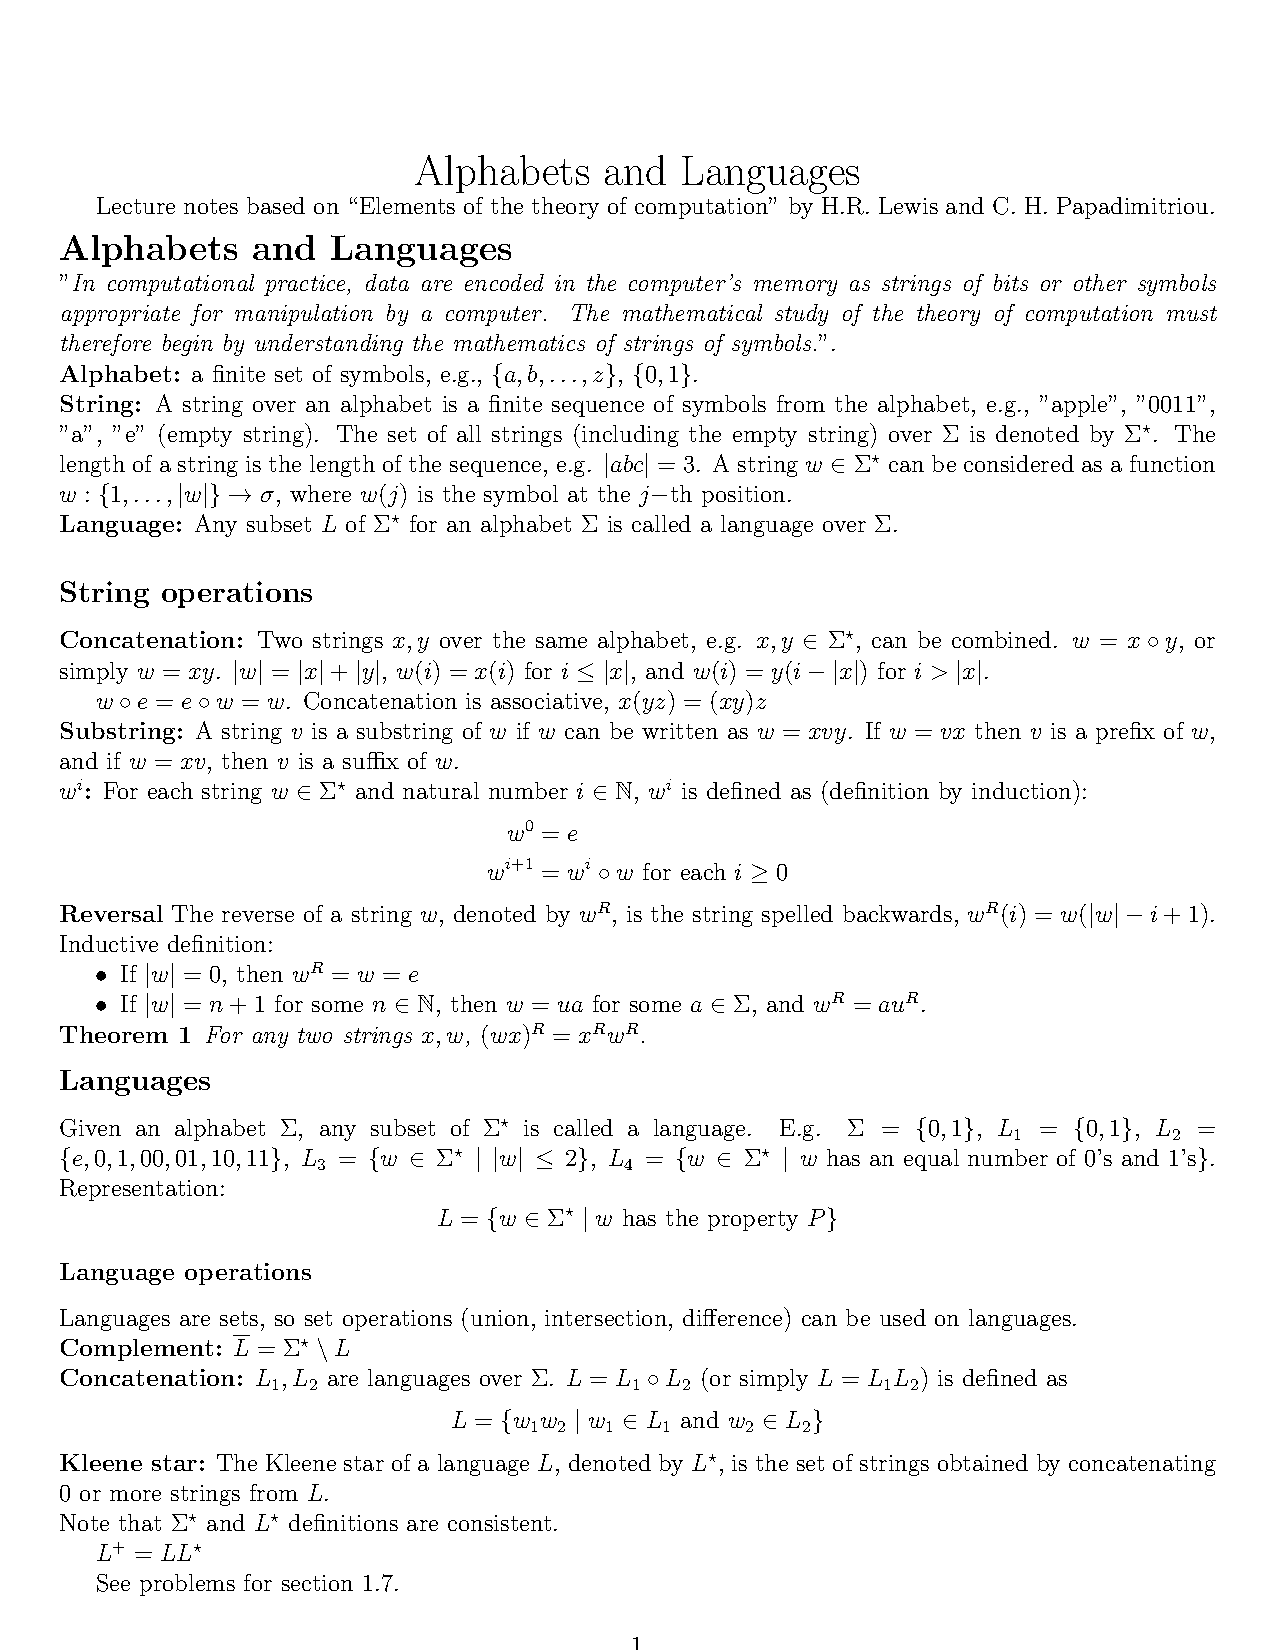
\includepdf{notes/chapter_1.2-alphabets-and-languages.pdf}

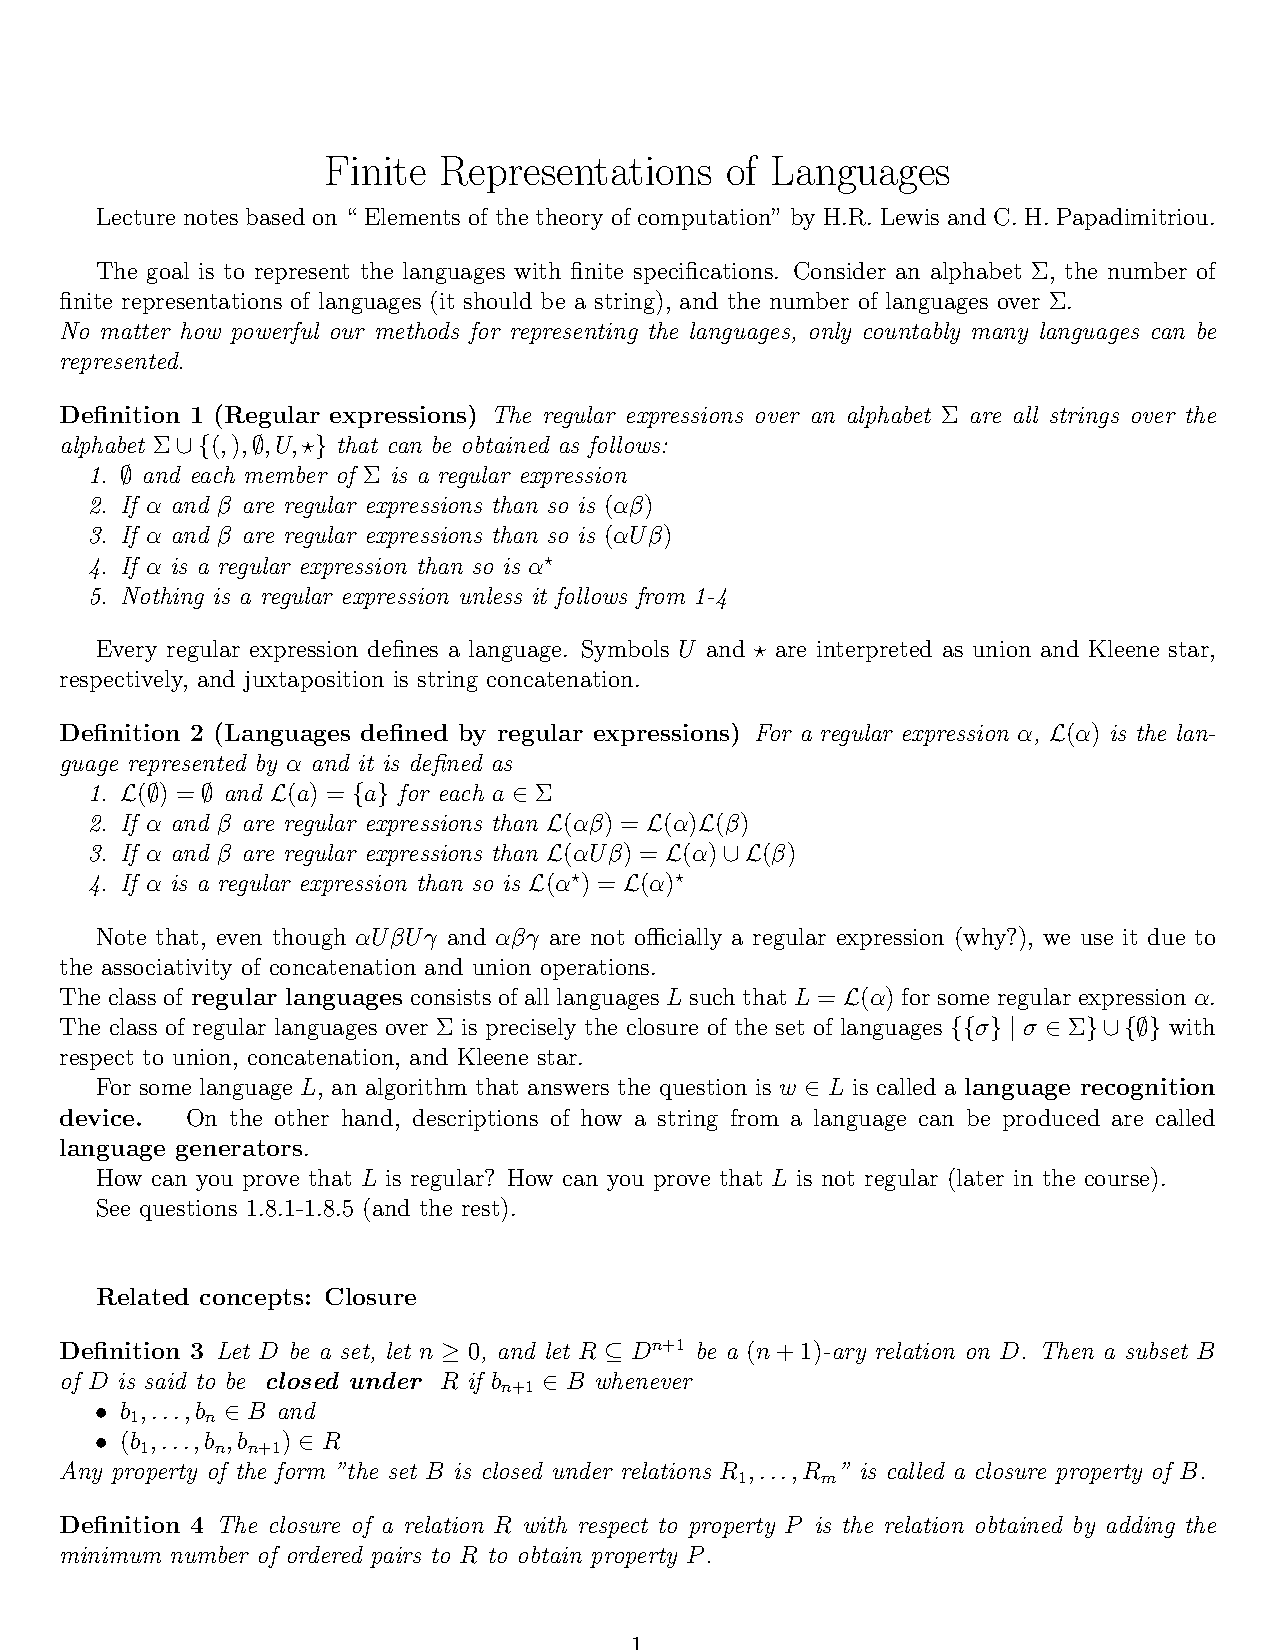
\includepdf{notes/chapter_1.3-finite-representations-of-languages.pdf}

\end{document}
